\section{Solution Proposal}
\label{sec:solution-proposal}
In this section I'll describe the architecture for the agent.

\subsection{Architecture}
\ac{DST} is divided into two parts.
The first one, the engine, is written in C++ and isn't public (we only have access to the binaries).
The second on, the content, is written in Lua scripts and is available publicly (to whoever has a copy of the game).

Through the creation of a mod\footnote{Modding is a growing practice in games which consists in altering the game's original content.}, I'll be able to introduce a new character in the game that will in fact be a social autonomous agent.
This is in fact the best way we can achieve this, since the game already works with a platform for the sharing of mods created by the community, Steam Workshop\footnote{Steam Workshop is a content sharing platform. https://steamcommunity.com/workshop/}.

\ac{DST} content is composed by entities.
These entities are made up of four different parts: Prefabs, Components, Stategraphs, and Brains.

Prefabs and Components are the meat and potatoes of any entity in the world.
Simply put, prefabs are what a thing \textit{is}, while Components are what a thing \textit{does}.

Lets look at the firepit as an example.
What \textit{is} it?
A firepit!
So it becomes a \textit{firepit} Prefab.
What does it \textit{do}?
It gets built, and it burns, and takes fuel, and can be looked at, and produces light...
So we don't make a \textit{firepit} component, instead we have a \textit{burnable} component, and a \textit{fueled} component, and so forth.

\begin{figure}
  \centering
    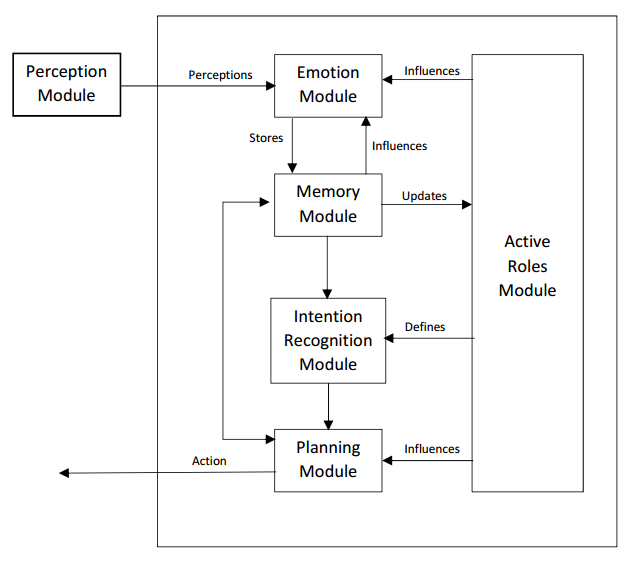
\includegraphics[width=.75\textwidth]{walter-architecture}
  \caption{The agent's architecture.}
  \label{fig:walter-architecture}
\end{figure}

This means that Components are where all the work happens, all the logic and data storage.
A Prefab is an instruction that says which Components to use and how to configure them, e.g. both the firepit and the campfire have a "fueled" component, but the firepit can take more fuel than the campfire.

Stategraphs are mainly used for controlling animation and timing.
Brains are used for AI and decision-making so only the most complex creatures use them.
Brains make use of a commonly used (in games) technique called Behaviour Trees.

Generally each behaviour in the tree boils down to sending instructions to components.
Components still end up doing all the real "work".
The \textit{ChaseAndAttack} behaviour, for example, sends instructions to the Locomotor (for movement) and Combat (for attacking) components, and those components handle the details.

This architecture is heavily based on Dorgoly's architecture, described in \ref{sec:dorgoly}.
Therefore it will also have an Emotion Module, a Memory Module, an Intention Recognition Module, a Planning Module, and a Active Roles Module (check Fig. \ref{fig:walter-architecture}.
The main difference will be the division of the Event Handler Module into two different modules: Perception Module and Planning Module.
While the former will be in charge of handling the perception of the environment and events in the environment, e.g. another player attacked the agent's basecamp by destroying a chest, the latter will take care of the action taking part.

These modules will be implemented as Components since they define what the character \textit{does}.
I'll then use the Brains of an entity to trigger the process of choosing an action.

\subsection{Evaluation}
There will be two main points to evaluate in this work: the player's game play experience after playing with the agent and the agent's capabilities to survive in \ac{DST}.

To find out if the player's experience has changed, a game playing session followed by a questionnaire is the best option.
However, given that \ac{DST} has such an open game play experience, players may choose not to interact with the agent.
So it is necessary to give some guidelines to testers.

One good way to get more feedback will be the sharing of the mod with the online community.
By doing so, more experienced and veteran players can test and give feedback on the agent and their experience.

The second part of evaluation is not directly related to this work's objectives, but is an important aspect of the agent given that players may grow tired of an agent that does not play the game well.
This, and the fact that \ac{DST} has no end, makes the lifespan of the agent an interesting metric.

Through the comparison of this agent with another baseline agent\footnote{There was another agent developed for the original one-player game, Don't Starve, which can be watched in action here: https://youtu.be/9PnL-Mr9N4o} we can also try and understand if a social agent has better results than a simple reactive agent (in terms of longevity).

\subsection{Planning}
\begin{figure}
  \centering
    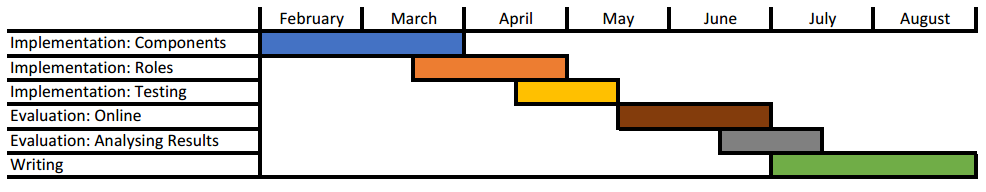
\includegraphics[width=\textwidth]{gantt}
  \caption{Gantt chart depicting the planning for the remainder of the work.}
  \label{fig:gantt}
\end{figure}
The realization of this work will be divided in two main parts: development and evaluation.
First of all, I'll implement the agent.
For this I make an estimate of about three to four months, from February until the middle of May.
Then I'll evaluate the agent by making it available to the community and leave it up for feedback for about a month, June.
Finally, I'll reserve the final two months for writing the final document, July and August.

